\documentclass[12pt]{article} 

\usepackage{datetime} 
\usepackage{graphicx}
\usepackage{wrapfig}
\usepackage[superscript,biblabel]{cite}
\usepackage{tocloft}
\usepackage{float}
\usepackage{subfig}		% handles subfloats
\usepackage{caption}
\usepackage{amssymb,amsmath}
\usepackage[hypcap]{caption}
\usepackage{framed}
\usepackage{verbatim}
\usepackage[numbers,square]{natbib}
\usepackage{listings}


\usepackage[utf8]{inputenc} % input encoding; lahko je tudi [cp1250] ali [latin2

% za vlkjučevanje literature na kazalu
\usepackage[nottoc,numbib,notlof]{tocbibind}


\renewcommand{\contentsname}{Kazalo}
\renewcommand{\figurename}{Graf}
\renewcommand{\listfigurename}{Kazalo slik in tabel}
\renewcommand{\abstractname}{Povzetek}
\renewcommand{\bibname}{Literatura}


\oddsidemargin = 31pt
%\textwidth = 430pt

\topmargin = 2pt
\headheight = 0pt
\hoffset = 0pt
\headsep = 0pt
\textheight = 600pt

%\intextsep = 0pt
% Začetek dokumenta 
\begin{document} 
	
%Naslovna stran
\begin{titlepage}
\begin{center}

%Za kodo .c 

\lstset{
numbers=left, 
numberstyle=\small, 
numbersep=8pt, 
frame = single, 
language=Pascal, 
framexleftmargin=15pt}

~\\[8cm]

{\LARGE List of functions : FreeRTOS - WIZ820io}\\[1cm]


\vfill
Ljubljana, 10. Julij 2014\\[2.7cm]



\end{center}
\end{titlepage}

\section{Uvod}
FreeRTOS aplikacije se poganjajo kot vse ostale, dokler ne pokličemo ukaza vTaskStartScheduler(), ki ga ponavadi kličemo iz “main()“. Preden uporabljamo funkcije RTOS-a se je dobro prepričati, da delujejo vse funkcije za izbrano tarčo?. FreeRTOS je zgrajen okoli treh glavnih C datotek 
\begin{itemize}
	\item tasks.c - kjer so rutine za ustvarjanje nalog, etc. 
	\item queue.c - kjer so rutine za manipulacijo z nalogami (blokiranje, pošilanje v ozadje, ...)
	\item list.c - ?
	\item portable/[compiler]/[architecture]/port.c  
\end{itemize}
Glavne mape, ki jih moramo vključiti pri prevajanju sta \textbf{Source/include} in \textbf{Source/portable/[compiler]/[architecture]}. Vsak projekt mora vsebovati tudi konfiguracijsko datoteko “FreeRTOSConfig.h”, kjer so definirane rutine in spremenljivke, ki temeljijo na namembnosti našega projekta. 
Najlažji način za ustvarjanje novih aplikacij je, da iz strani \textit{www.freertos.org} povlečemo source in v mapi \textbf{Demo} poiščemo ustrezno mapo za našo tarčo. Nato najprej prevedemo projekt in ga preizkusimo na naši tarči. Ko smo se prepričali, da deluje, lahko nadaljujemo z nadgrajevanjem demo primera na željeni projekt. \newline
Struktura funkcije \textbf{main()} bi naj izgledala takole
\begin{figure}[h]
 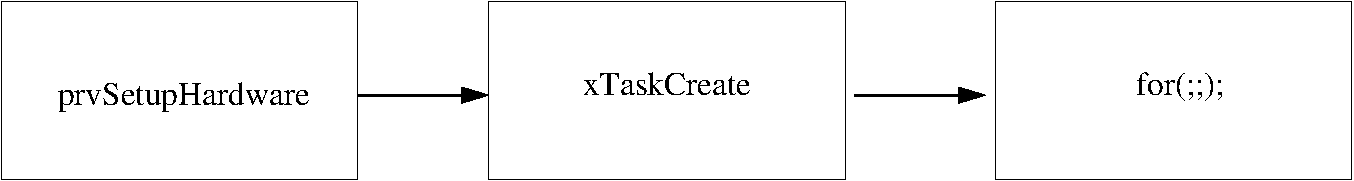
\includegraphics[scale=0.6]{main.pdf}
\end{figure}
\section{Interrupts - interupti}
Interrupti so lahko bodisi strojni - zunanji bodisi programerski. Definiramo jih s pomočjo NVIC strukture. Pri tem moramo vključiti ustrezne header datoteke. Nastaviti moramo kateri kanalo opazujemo, kakšne prioritete ima naš interrupt, ter ga seveda omogčiti. 
\begin{lstlisting}[frame = single]
NVIC_InitStruct.NVIC_IRQChannel = EXTI0_IRQn;
NVIC_InitStruct.NVIC_IRQChannelPreemptionPriority = 0x1;
NVIC_InitStruct.NVIC_IRQChannelSubPriority = 0x0;
NVIC_InitStruct.NVIC_IRQChannelCmd = ENABLE;
\end{lstlisting} 
V kolikor želimo uporabiti zunanji interrupt moramo prej definirati zunanj interupt na EXTI vodilu.
\begin{lstlisting}[frame = single]
EXTI_InitStruct.EXTI_Line = EXTI_Line0;
EXTI_InitStruct.EXTI_Mode = EXTI_Mode_Interrupt;
EXTI_InitStruct.EXTI_Trigger = EXTI_Trigger_Falling;
EXTI_InitStruct.EXTI_LineCmd = ENABLE;
\end{lstlisting}
Ob dogodku na vodilu se potem pokliče funkcija \textbf{EXTIn\_IRQHandler(void)} v katero moramo definirati in v njej počisti interrupt flag in nato naredimo, kar želimo ob določenem interruptu. 
Naloge so v FreeRTOS osrednji del strukture programa. Nalogo ustvarimo s klicem \textbf{vTaskCreate}, kjer določimo, nalogo, njeno ime, prioriteto, parametre ki jih želimo podati in TaskHandle. 
Naloge - Tasks so lahko v štirih stanjih
\begin{itemize}
 \item running : kadar se naloga izvršuje 
 \item ready : so tiste naloge, ki čakajo na izvršitev, ker se trenutno izvršuje naloga z enako oziroma višjo prioriteto
 \item blocked : kadar naloga čaka na nek zunanji dogodek ali podatek oziroma sprostitev semaforja oz. čakalne vrste. 
 \item suspended : v tem stanju je naloga samo kadar kličemo \textbf{vTaskSuspend()}. Iz tega stanja je mogoče priti samo z \textbf{vTaskResume()}
\end{itemize}
\section {Queues - čakalne vrste}
Komunikacija med nalogami poteka s pomočjo čakalnih vrst. Med nalogami lahko pošiljamo in sprejemamo vrednosti lokalnih spremenljivk s pomočjo \textbf{ xQueueSend} in \textbf{ xQueueRecive}. 
\section{Semaphores - semaforji}
Semaforji so nadgradnja čakalnih vrst (Queue) in se uporabljajo za sinhronizacijo med nalogami, kot tudi znotraj nalog. Za sinhronizacicijo mend nalogami  ustvarimo \textbf{xSemaphoreCreateBinary()}. Lahko bi uporabili tudi \textbf{xSemaphoreCreateMutex()}, vendar v dokumentaciji pri uporabi ISR slednjega ne priporočajo. Dostop do določenega dela programa blokiramo s funkcijo
\begin{lstlisting}[frame = single ]
xSemaphoreTake(xSemaphoreHandle, TickType_t);	
\end{lstlisting}
ki ga blokira dokler ga ne sprostimo s funkcijo 
\begin{lstlisting}[frame = single ]
xSemaphoreGive(xSemaphoreHandle);	
\end{lstlisting}
Spet se je pri uporabi ISR bolje poslužiti \textbf{xSemaphoreTakeFromISR} in \textbf{xSemaphoreGiveFromISR}. \footnote{Primer Echo TCP serverja, ki komunicira preko SPI s pomočjo DMA ne deluje, saj je iz neznanega razloga prioriteta veliko nižja kot prioriteta trenutne naloge in zaradi tega obstane v zanki znotraj funkcije \textbf{xSemaphoreGiveFromISR}.}
\section{ Echo TCP server }
Preprost Echo TCP server ustvari en socket in čaka na klienta, da se poveže. Ob vzpostavitvi povezave ne naredi ničesar. Ob prejemu podatkov pa vrne iste podatke. Če so podatki enaki 'quit' zapre socket in pošlje nalogo v spanje. TCP server je nadgradnja demo primera iz git repozitorija \\
 \textit{git://github.com/vagabondtt1503/STM32F4-Discovery-FreeRTOS-GCC.git}. Dodamo mu  dve novi datoteki s funkcijami za upravljanje z Wiznet modulom in TCP protokolom (spi.c, W5200.c) in prilagodimo \textbf{main.c}.  
\subsection{main.c}
Najprej vključimo header datoteke, ki jih potrebujemo za naš server in definiramo prototip naloge. 
\begin{lstlisting}[frame = single ]
#include "spi.h"
#include "W5200.c"
void set_macTask(void *  pvParameters)
\end{lstlisting}  
Funkciji \textbf{main()} dodamo nov task
\begin{lstlisting}[frame = single ]
xTaskCreate(set_macTask, 
		"SETMAC", 
		configMINIMAL_STACK_SIZE, 
		NULL, mainFLASH_TASK_PRIORITY, 
		&set_macTaskHandle);
\end{lstlisting}  
V funkcijo \textbf{prvSetupHardware} dodamo našo funkcijo, ki nastavi strojno opremo za prenos podatkov preko SPI vodila in interrupte. 
\begin{lstlisting}[frame = single]
static void prvSetupHardware(void)
{
	.....
	
	init_SPI1();
	
	....
}
\end{lstlisting}
Nazadnje še določimo nalogo. Najprej je potrebno inicializirati wiznet, mu nastaviti mac naslov, ip naslov, gateway in masko. 
\begin{lstlisting}[frame = single ]
uint8_t address[6] = {0xdd,0xaa,0xbb,0xcc,0x11,0x22}; 
const  uint8_t ip[4] = {0xc0, 0xa8, 0x0, 0x08};
const uint8_t subnet[4] = {0xff,0xff,0xff,0x0};
const uint8_t gw[4] = {0xc0, 0xa8, 0x0, 0x01};

wiznet_initialize();	
wiznet_configure_network(ip, subnet, gw);
wiznet_set_hardware_address(address);

\end{lstlisting}
Sedaj ustvarimo socket na portu 80, nastavimo wiznet v način poslušanja.

\begin{lstlisting}[frame = single]	
/*create socket and send byte */
uint8_t s;
s = socket(W5200_Sn_MR_TCP, 80, 0);
uint8_t buf [100]; 
listen(s);
\end{lstlisting}
Naloga tukaj vstopi v neskončno zanko, kjer pošlje sama sebe v spanje, dokler se ne zgodi dogodek na zunanjem pinu, ki smo ga določili v “spi.c“. Ob dogodku, določi kakšen dokodek se je zgodil in v primeru prejema podatkov prejme podatke in jih pošlje nazaj. 
\begin{lstlisting}[frame = single]
int len;
for( ;; )
{
  /*we are now listening
  suspend task set_macTask()*/
  vTaskSuspend(set_macTaskHandle);
  len = recv(s, buf, 100, 0);

  if ( !strncmp(buf, "quit", 4))
  {
    uint8_t * r = "Bye\n"; 
    send(s, r, 4,0);
    closesocket(s);
  } 
  send(s, buf, len, 0);
}
vTaskDelete( NULL );

\end{lstlisting}

\subsection{W5200.c}
Dogodek na zunanjem pinu (interrupt wizneta) je v “spi.c“ definiran tako, da požene funkcijo \textbf{void EXTI0\_IRQHandler(void)}. Kjer najprej preverimo, če se je res zgodil dogodek, nato iz wiznet registra preberemo na katerem socketu in kateri interrupt se je zgodil, ter sporočimo, da smo obdelali interrupt. 
\begin{lstlisting}[frame = single]
void EXTI0_IRQHandler(void) //EXTI0 ISR
{
  // cehck if EXTI line is asserted 
  if(EXTI_GetITStatus(EXTI_Line0) != RESET) 
  {  
  //clear interrupt
  EXTI_ClearFlag(EXTI_Line0); 
  locate_interrupt();
  }  
}

void locate_interrupt()
{
  uint8_t code = 0x4; 
  spi_read(W5200_IMR2, 1, &code);
  spi_read(W5200_Sn_IR(code), 1, &code);

  spi_dma_sendByte(W5200_Sn_IR(0x0), 0xff);
  switch (code )
  {  
    case 0x1: 
	// connection established 
	// do nothing wait for input. 
	break;
    case 0x2:
	break;
    case 0x4:
	// recived data resume task
	vTaskResume(set_macTaskHandle); 
	break;
    default:
	break;		
  }
}
\end{lstlisting}

\subsection{spi.c}
V tej datoteki je inicializacijska funkcija SPI, kjer definiramo vse pine, ki jih SPI uporablja. Definirani so interrupti in nekatere funkcije, ki se sprožijo ob interruptih. Poleg tega so v tej datoteki funkcije za branje registrov preko SPI vodila. 

\end{document}
